% !TeX program = pdflatex
% !TeX encoding = UTF-8
%=======================================================================
%  GRIS-NOT-001  ·  Plantilla de notas rápidas para la memoria
%  Proyecto 00503 - Generator inspection robotic system · Mecanalisis
%  Identidad: GRIS-IDENTIDAD-001 v1.4
%-----------------------------------------------------------------------
%  CÓMO USARLA (en 3 pasos)
%
%   1. Copiá este archivo con el código de la nota:
%         memoria/notas/02489-00-MC007.tex
%      El número (###) es correlativo: mirá la última nota y sumá uno.
%
%   2. Completá los cuatro datos del bloque «DATOS DE LA NOTA».
%
%   3. Escribí:
%        · Resultados (obligatorio, siempre primero): lo que se sabe
%          ahora que antes no se sabía. Frases cortas, con números.
%        · El resto es libre. Usá los títulos que te sirvan, o ninguno.
%
%   Compilar:  pdflatex 02489-00-MC007.tex
%   En Overleaf: subí el .tex y logo-gris.pdf.
%
%  LOGO: se usa «logo-gris.pdf» (GRIS-LOGO-003, reducido) de esta carpeta
%  o de ../plantilla/. Si falta, se escribe «GRIS» como marcador.
%=======================================================================
\documentclass[11pt,a4paper]{article}

%=======================================================================
%  DATOS DE LA NOTA  ← lo único que hay que tocar arriba
%=======================================================================
\newcommand{\codigo}{02489-00-MC001}          % 02489-00-MC###
\newcommand{\titulo}{Torque admisible de los engranajes cónicos de la rueda}
\newcommand{\autor}{Matías Gaviño}
\newcommand{\fecha}{24/09/2026}                    % o p. ej. {24/09/2026}

%=======================================================================
%  ESTILO  (no hace falta tocar nada de aquí hasta \begin{document})
%=======================================================================
\usepackage[T1]{fontenc}
\usepackage[utf8]{inputenc}
\usepackage[spanish,es-noshorthands,es-tabla]{babel}
\usepackage{lmodern}
\usepackage[a4paper,top=3.0cm,bottom=2.4cm,left=2.4cm,right=2.4cm,
            headheight=20pt,headsep=1.2cm,footskip=1.1cm]{geometry}
\usepackage{microtype}
\usepackage{xcolor}
\usepackage{graphicx}
\usepackage{booktabs}
\usepackage{array}
\usepackage{enumitem}
\usepackage{titlesec}
\usepackage{fancyhdr}
\usepackage{caption}
\usepackage[hidelinks]{hyperref}

% --- colores -----------------------------------------------------------
\definecolor{gris-naranja}{HTML}{FF7A00}   % naranja institucional
\definecolor{tinta}{HTML}{1E2328}
\definecolor{gris-medio}{HTML}{6B7280}
\definecolor{gris-linea}{HTML}{DADDE1}
\color{tinta}

\hypersetup{pdftitle={\codigo\ -- \titulo}, pdfauthor={\autor},
            colorlinks=true, linkcolor=tinta, urlcolor=tinta}

% --- logo ---------------------------------------------------------------
\graphicspath{{./}{../plantilla/}{plantilla/}}
\newcommand{\logogris}{%
  \IfFileExists{logo-gris.pdf}
    {
\includegraphics[height=16pt]{logo-gris.pdf}}
    {\IfFileExists{../plantilla/logo-gris.pdf}
      {
\includegraphics[height=16pt]{../plantilla/logo-gris.pdf}}
      {{\fontsize{18}{18}\selectfont\bfseries\sffamily\color{gris-naranja}GRIS}}}}

% --- tipografía del cliente (código documental) --------------------------
% Geogrotesque no es libre; se usa Roboto Condensed Bold, que viene con
% TeX Live y Overleaf y tiene el mismo aire que el logo.
\newcommand{\fuentecliente}{\fontfamily{Roboto-TLF}\fontseries{bc}\selectfont}

% --- encabezado y pie ---------------------------------------------------
\pagestyle{fancy}
\fancyhf{}
\renewcommand{\headrulewidth}{0.4pt}
\renewcommand{\headrule}{\vspace{3pt}{\color{gris-linea}\hrule height \headrulewidth}}
\fancyhead[L]{\logogris}
\fancyhead[R]{{\fuentecliente\fontsize{12}{12}\selectfont\color{gris-medio}\codigo}}
\fancyfoot[R]{\footnotesize\color{gris-medio}\thepage}

% --- títulos numerados ----------------------------------------------------
\setcounter{secnumdepth}{2}
\titleformat{\section}{\large\bfseries}{\thesection}{0.8em}{}
\titleformat{\subsection}{\normalsize\bfseries}{\thesubsection}{0.8em}{}
\titlespacing*{\section}{0pt}{16pt}{5pt}
\titlespacing*{\subsection}{0pt}{11pt}{3pt}

% --- texto ------------------------------------------------------------------
\setlength{\parindent}{0pt}
\setlength{\parskip}{6pt}
\linespread{1.05}
\setlist{topsep=2pt, itemsep=2pt, parsep=0pt, leftmargin=1.2em}
\setlist[itemize]{label={\raisebox{0.15ex}{\small$\bullet$}}}
\captionsetup{font={small,color=gris-medio}, labelfont=bf, skip=5pt}
\renewcommand{\arraystretch}{1.25}

% --- cabecera de la nota ------------------------------------------------------
\newcommand{\cabecera}{%
  \thispagestyle{fancy}%
  {\fontsize{20}{24}\selectfont\bfseries\titulo\par}%
  \vspace{5pt}%
  {\small\color{gris-medio}\fecha\quad·\quad\autor\par}%
  \vspace{6pt}}

% --- ayudas opcionales --------------------------------------------------------
% \figura{archivo}{ancho}{pie}
\newcommand{\figura}[3]{%
  \begin{figure}[htbp]\centering
    \includegraphics[width=#2\linewidth]{#1}\caption{#3}
  \end{figure}}

% --- paquetes adicionales de esta nota --------------------------------------
\usepackage{amsmath}
\usepackage{float}
\usepackage{tabularx}
\usepackage{xspace}
\graphicspath{{02489-00-MC001/figuras/}}
\newcommand{\Nm}{\,N\,m\xspace}

%=======================================================================
\begin{document}
\cabecera

%-----------------------------------------------------------------------
%  RESULTADOS  (siempre primero, lo único obligatorio)
%-----------------------------------------------------------------------
\section{Resultados}
Torque admisible por engranaje del par cónico 1:1 a 90° de la rueda, según Shigley
(cap.~15, método AGMA), con confiabilidad del 95\,\%, torque en ambos sentidos y 10~años de uso.
Todas las mejoras respetan $d_a\le11{,}5$~mm.

\begin{table}[H]\centering\small\setlength{\tabcolsep}{4.5pt}
\begin{tabular}{l r ccc cc r}
\toprule
 & & \multicolumn{3}{c}{Torque normal [N\,m]} & \multicolumn{2}{c}{Pico de 10 s [N\,m]} & \\
\cmidrule(lr){3-5}\cmidrule(lr){6-7}
Diseño & $d_a$ [mm] & 0,5 rpm & 50 rpm & 100 rpm & 0 rpm & 100 rpm & vs.\ actual\\
\midrule
KG M50S20, S45C (actual)          & 10,71 & 0,129 & 0,083 & \textbf{0,076} & 0,195 & \textbf{0,133} & 1,0\\
KG M50B20, latón                  & 10,71 & 0,063 & 0,040 & 0,039 & 0,094 & 0,065 & 0,5\\
m\,0,5 z20, SCM440 300 HB         & 10,71 & 0,206 & 0,133 & \textbf{0,128} & 0,311 & \textbf{0,213} & 1,7\\
m\,0,5 z20, SCM415 carburizada    & 10,71 & 0,408 & 0,263 & \textbf{0,254} & 0,615 & \textbf{0,421} & 3,3\\
m\,0,6 z17, SCM415 carburizada    & 11,05 & 0,482 & 0,310 & \textbf{0,299} & 0,725 & \textbf{0,496} & 3,9\\
\bottomrule
\end{tabular}
\end{table}

\begin{itemize}
  \item \textbf{Mitra actual KG M50S20:} admite \textbf{0,076\Nm} en servicio continuo y
        \textbf{0,133\Nm} en picos, a 100~rpm.
  \item \textbf{Datasheet de KG:} publica 1,5~W a 100~rpm (0,143\Nm). Recalculado con Shigley \emph{en las mismas
        condiciones del datasheet} da 0,071\Nm a flexión y 0,047\Nm a picado: \textbf{el datasheet da el doble} que
        Shigley y no publica el picado, que es el límite real. Con su propia regla de carga en ambos sentidos (2/3),
        KG daría 0,095\Nm, un 25\,\% más que esta nota.
  \item \textbf{No hay mejora de stock dentro de 11,5~mm:} la siguiente mitra KG (M50S25) mide 13,2~mm.
  \item \textbf{Mejora sin cambiar la geometría:} la misma mitra m\,0,5 z20 a medida en SCM440 bonificado (×1,7)
        o en SCM415 carburizado (×3,3). Entra en el mismo lugar que la actual.
  \item \textbf{Máximo dentro de 11,5~mm:} m\,0,6 z17 carburizada (×3,9; 0,299\Nm continuo). Es el mayor módulo
        que entra con los 16 dientes mínimos, pero cambia la distancia de montaje.
  \item Por encima de 0,28\Nm de pico los dos prisioneros M2,5 ya no alcanzan: las mejoras necesitan arrastre
        positivo (plano en D o pasador) y, las carburizadas, eje de 4~mm. Todo vale solo con \textbf{grasa EP}.
\end{itemize}

\begin{figure}[H]\centering
  
\includegraphics[width=\linewidth]{fig_resumen.pdf}
  \caption{Torque admisible de cada diseño en servicio normal y en picos de 10~s.}
  \label{fig:resumen}
\end{figure}

%-----------------------------------------------------------------------
\section{Datos y supuestos}
El par transmite el giro de un motor BLDC a la rueda de un carro, con ejes a 90° y relación 1:1.

\begin{table}[H]\centering\small
\begin{tabularx}{\linewidth}{l X l}
\toprule
Dato & Valor & Origen\\\midrule
Par & Cónicos rectos iguales (mitras), 1:1, $\Sigma=90^\circ$ & pedido\\
Envolvente & $d_a\le11{,}5$~mm para las mejoras (la actual mide 10,71~mm) & pedido\\
Velocidades & 0; 0,5; 50 y 100 rpm & pedido\\
Confiabilidad & $R=0{,}95$ & pedido\\
Uso & 20 h seguidas por mes; vida de 10 años (2400 h) & pedido / \textbf{supuesto}\\
Carga & BLDC con perfil trapezoidal suave; torque en ambos sentidos & pedido\\
Picos & 10 s cada uno, 1 por hora de uso (2400 en la vida) & pedido / \textbf{supuesto}\\
Lubricación y temperatura & Grasa en compartimiento cerrado; 30--40\,°C & pedido\\
Montaje & Ambos engranajes en voladizo & \textbf{supuesto} (conservador)\\
\bottomrule
\end{tabularx}
\end{table}

\paragraph{Ciclo de carga.}
El torque cambia de sentido (adelante, atrás, aceleración y frenado), así que cada diente se flexiona hacia
los dos lados: se usa el 70\,\% de la resistencia a flexión (Shigley, «Carga invertida», sec.~15-2).
El servicio normal dura toda la vida, $n_{normal}=n\cdot60\cdot20\cdot12\cdot10$ ciclos. Cada pico suma
$\max(1;\,n\cdot10/60)$ ciclos. Los dos regímenes se combinan con la regla de Miner, con la mitad del daño para cada uno:
\begin{equation}
\frac{n_{normal}}{N_{normal}}+\frac{n_{pico}}{N_{pico}}=0{,}5+0{,}5=1
\quad\Rightarrow\quad N_{eval}=2\,n .
\end{equation}

%-----------------------------------------------------------------------
\section{Comparación con el datasheet de KG}
KG publica, para sus mitras de S45C, una tabla de potencia admisible a flexión según la velocidad. La columna de
resistencia superficial (picado) figura con «--»: no la publica.

\begin{figure}[H]\centering
  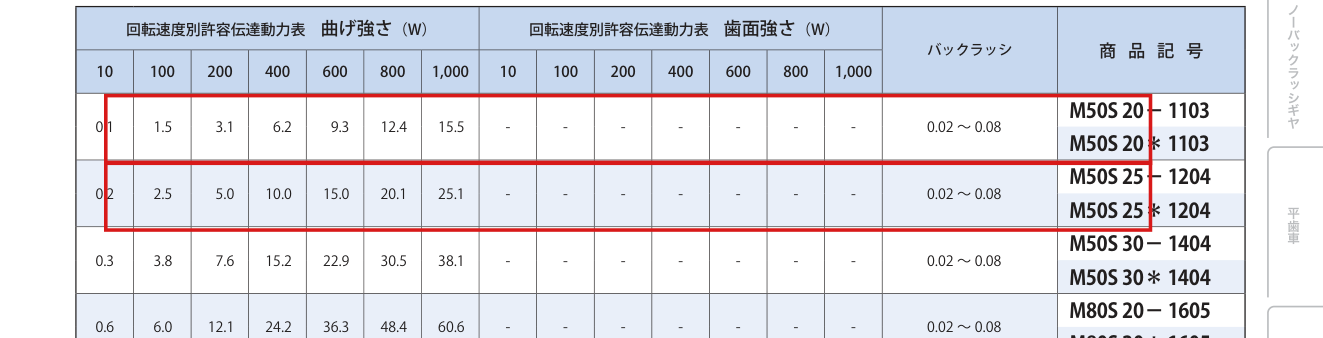
\includegraphics[width=\linewidth]{kg_datasheet_potencia.png}
  \caption{Datasheet KG: potencia admisible a flexión (W) y a picado («--») por velocidad. M50S20: 1,5~W a 100~rpm;
  M50S25: 2,5~W. \emph{Fuente: KG, catálogo KG4001, p.~261.}}
\end{figure}

\begin{table}[H]\centering\small
\begin{tabularx}{\linewidth}{l X X}
\toprule
Condición & Datasheet KG (KG5001, p.~18) & Esta nota\\\midrule
Norma & JGMA 403-01 / 404-01 (alcance: $m\ge1{,}5$) & Shigley cap.~15 (ANSI/AGMA 2003-B97)\\
Modos publicados & Solo flexión & Flexión y picado\\
Ciclos & $\ge10^7$, $K_L=1$ & $2{,}9\times10^7$ (Miner) a 100~rpm\\
Choque & Moderado, $K_O=1{,}25$ & Motor suave, $K_A=1{,}0$\\
Confiabilidad & $K_R=1{,}2$; $C_R=1{,}15$ & $R=0{,}95$: $Y_Z=0{,}895$; $Z_Z=0{,}946$\\
Sentido de carga & Uno solo; con inversión, 2/3 del valor & Ambos sentidos: 70\,\%\\
Lubricación & Baño de aceite 100~cSt & Grasa EP\\
Montaje & Ambos en voladizo & Ambos en voladizo\\
Ancho de diente & El de catálogo (2,5~mm) & Útil $0{,}3R_e=2{,}12$~mm\\
\bottomrule
\end{tabularx}
\end{table}

\paragraph{Mismas condiciones.} Para ver si el método coincide, se recalculó con Shigley usando las condiciones del
datasheet ($K_A=1{,}25$, $Y_Z=1{,}2$, $Z_Z=1{,}15$, $10^7$ ciclos, un sentido):

\begin{table}[H]\centering\small\setlength{\tabcolsep}{5pt}
\begin{tabular}{l r c c c c c}
\toprule
Mitra & rpm & Datasheet KG & \multicolumn{3}{c}{Shigley, condiciones KG [N\,m]} & Shigley / KG\\
\cmidrule(lr){4-6}
 & & N\,m & Flexión & Flexión, $b$ total & Picado & (flexión)\\
\midrule
M50S20 & 100  & 0,143 & 0,071 & 0,084 & 0,047 & 0,50\\
       & 1000 & 0,148 & 0,065 & 0,077 & 0,043 & 0,44\\
M50S25 & 100  & 0,239 & 0,119 & 0,135 & 0,095 & 0,50\\
       & 1000 & 0,240 & 0,108 & 0,122 & 0,087 & 0,45\\
\bottomrule
\end{tabular}
\end{table}

\begin{figure}[H]\centering
  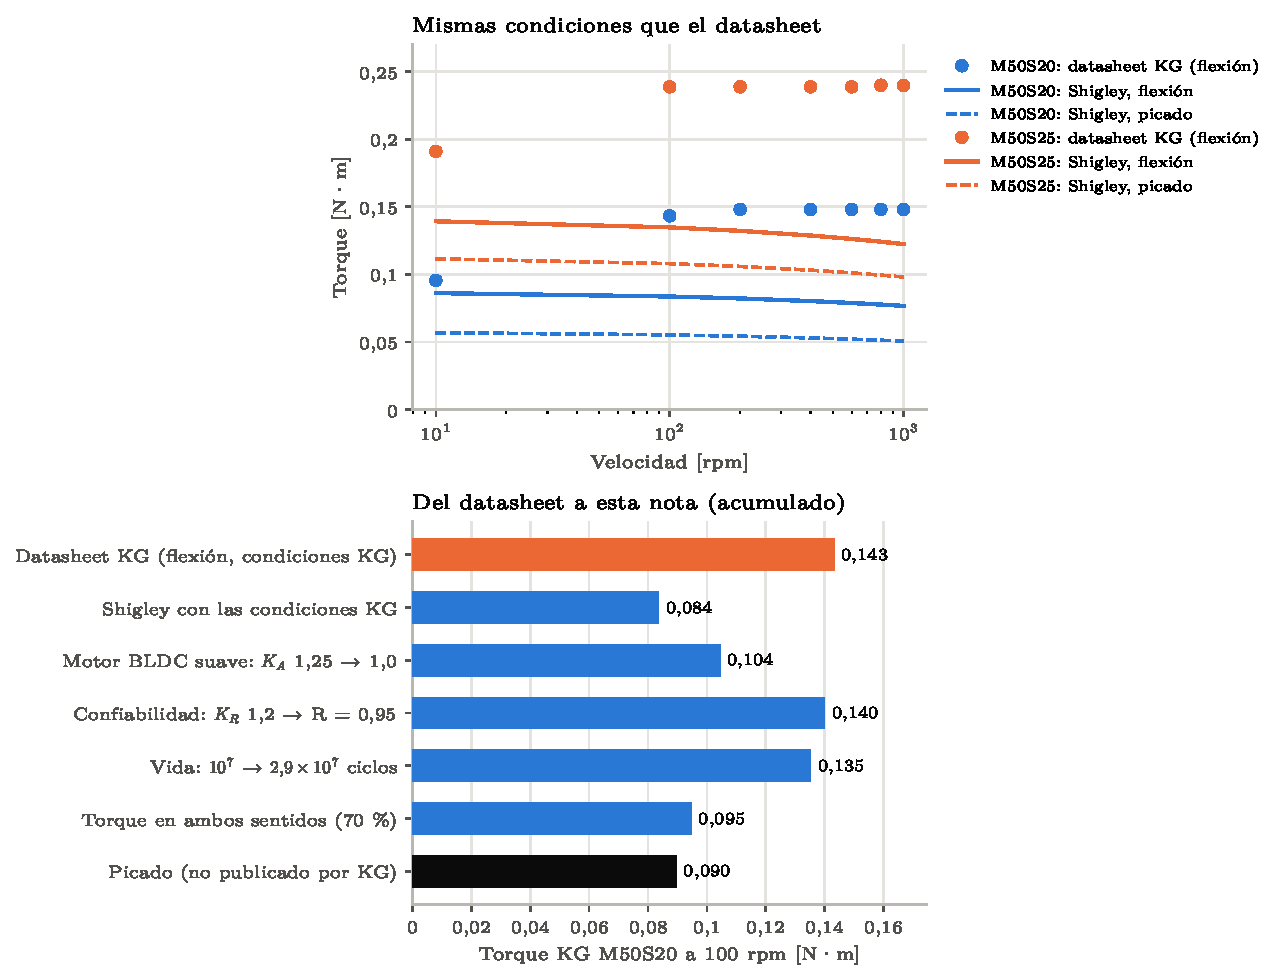
\includegraphics[width=\linewidth]{fig_datasheet.pdf}
  \caption{Arriba: datasheet KG frente a Shigley en las condiciones del datasheet. Abajo: del valor del datasheet al
  torque admisible de esta nota, cambiando una condición por vez.}
  \label{fig:datasheet}
\end{figure}

\begin{itemize}
  \item \textbf{Con las mismas condiciones, Shigley da la mitad} (0,44--0,50 entre 100 y 1000~rpm, en las dos mitras).
        El ancho explica solo una parte: acreditando los 2,5~mm completos se llega a 0,59. El resto es la diferencia
        entre JGMA y AGMA en resistencias admisibles y factores, y KG aplica JGMA 403 por debajo de su alcance ($m\ge1{,}5$).
        A 10~rpm la tabla da 0,1~W, un valor redondeado que no permite comparar.
  \item \textbf{El picado manda y KG no lo publica.} En las condiciones del datasheet, Shigley da 0,047\Nm a picado,
        un tercio del valor de la tabla. La tabla de KG no es un límite de uso para este par.
  \item \textbf{Del datasheet a esta nota} (fig.~\ref{fig:datasheet}, abajo): el método baja el valor de 0,143 a 0,071\Nm.
        El motor suave ($\times1{,}25$) y la confiabilidad del 95\,\% en lugar de $K_R=1{,}2$ ($\times1{,}34$) lo suben a 0,119.
        La vida más larga ($\times0{,}97$) y la carga en ambos sentidos ($\times0{,}70$) lo llevan a 0,080\Nm a flexión,
        y el picado fija el admisible en \textbf{0,076\Nm}.
\end{itemize}

%-----------------------------------------------------------------------
\section{Diseños analizados}
Para una mitra 1:1 de 20° Shigley pide al menos 16 dientes (tabla 13-3). Con $d_a=m(z+\sqrt2)\le11{,}5$~mm,
el mayor módulo normalizado posible es 0,6 (z16 o z17): m\,0,7 z16 ya mide 12,2~mm. Las mitras KG M50S25 (13,2~mm),
RS PRO 521-5780 (13,9~mm) y m\,0,6 z21 (13,4~mm) quedan fuera.

\begin{table}[H]\centering\small\setlength{\tabcolsep}{4pt}
\begin{tabular}{l l r r r r r r r}
\toprule
Diseño & Material & $m$ & $z$ & $d_e$ & $d_a$ & $b_{ef}$ & $Y_J$ & $Z_I$\\
 & & mm & & mm & mm & mm & & \\
\midrule
KG M50S20 & S45C, 170 HB & 0,5 & 20 & 10,0 & 10,71 & 2,12 & 0,200 & 0,062\\
KG M50B20 & Latón C3604B & 0,5 & 20 & 10,0 & 10,71 & 2,12 & 0,200 & 0,062\\
A medida & SCM440 bonificado 300 HB & 0,5 & 20 & 10,0 & 10,71 & 2,12 & 0,200 & 0,062\\
A medida & SCM415 carb. 58--62 HRC & 0,5 & 20 & 10,0 & 10,71 & 2,12 & 0,200 & 0,062\\
A medida & SCM415 carb. 58--62 HRC & 0,6 & 17 & 10,2 & 11,05 & 2,16 & 0,189 & 0,059\\
\bottomrule
\end{tabular}
\end{table}

\begin{itemize}
  \item \textbf{Geometría} ($\delta=45^\circ$): $d_e=mz$, $R_e=d_e/(2\sin\delta)$, $d_a=d_e+2m\cos\delta$.
        Shigley solo acredita un ancho útil $b_{ef}=\min(b;\,0{,}3R_e)$ (tabla 13-3); las mitras a medida se dimensionan con ese ancho.
  \item $Y_J$ y $Z_I$ salen de las figuras 15-7 y 15-6; para 17 dientes se interpolaron entre 16 y 20.
  \item \textbf{m\,0,5 z20 a medida:} misma geometría que la mitra actual, se reemplaza sin tocar la carcasa.
  \item \textbf{m\,0,6 z17:} gana un 18\,\% sobre la m\,0,5 z20 carburizada, pero su distancia de montaje es distinta.
\end{itemize}

%-----------------------------------------------------------------------
\section{Método}
Shigley, cap.~15, ecuaciones AGMA para cónicos rectos en unidades SI, con $W^t$ la fuerza tangencial en el diámetro exterior.
El torque admisible es el menor entre flexión y picado:
\begin{align}
\sigma_F &= \frac{W^t}{b}\,\frac{K_A K_v}{m_{et}}\,\frac{Y_x K_{H\beta}}{Y_\beta Y_J}
  \;\le\; \sigma_{FP}=\frac{0{,}70\,\sigma_{F\,\lim}\,Y_{NT}}{S_F\,K_\theta\,Y_Z}
  && \text{ec. (15-3), (15-4)}\\
\sigma_H &= Z_E\left(\frac{W^t}{b\,d_e\,Z_I}\,K_A K_v K_{H\beta} Z_x Z_{xc}\right)^{1/2}
  \;\le\; \sigma_{HP}=\frac{\sigma_{H\,\lim}\,Z_{NT}\,Z_W}{S_H\,K_\theta\,Z_Z}
  && \text{ec. (15-1), (15-2)}\\
T_{adm} &= \frac{d_e}{2}\,\min\!\left(W^t_F;\;W^t_H\right)
\end{align}

\begin{table}[H]\centering\small
\begin{tabularx}{\linewidth}{l c X}
\toprule
Factor & Valor & Criterio (Shigley 8.ª ed.)\\\midrule
$K_A$ sobrecarga & 1,00 & BLDC con perfil suave. Con golpes de rueda, 1,25 (fig.~\ref{fig:sens}).\\
$K_v$ dinámico & $\approx1{,}04$ & Ec. (15-5) y (15-6) con $Q_v=6$.\\
$Y_x$, $Z_x$ tamaño & 0,5 & Ec. (15-10) y (15-9): $m_{et}<1{,}6$ mm, $b<12{,}7$ mm.\\
$K_{H\beta}$ distribución & 1,25 & Ec. (15-11), $K_{mb}=1{,}25$: ambos en voladizo.\\
$Z_{xc}$ coronamiento & 2,0 & Ec. (15-12): sin coronamiento garantizado.\\
$Y_\beta$ curvatura & 1 & Ec. (15-13): dientes rectos.\\
$Y_{NT}$, $Z_{NT}$ ciclos & ec. & Ec. (15-15) y (15-14), figs.~15-9 y 15-8.\\
$Y_Z$, $Z_Z$ confiabilidad & 0,895 / 0,946 & Ec. (15-20) con $R=0{,}95$; $Z_Z=\sqrt{Y_Z}$.\\
$K_\theta$, $Z_W$ & 1 & Ec. (15-18) y (15-16): menos de 120\,°C, mismo material.\\
$S_F$, $S_H$ & 1 & Capacidad nominal; el margen lo dan $R$ y los supuestos.\\
\bottomrule
\end{tabularx}
\end{table}

\paragraph{Materiales.}
El S45C sin tratar entra como acero templado total grado~1 con 170~HB (mínimo de JIS G4051):
$\sigma_{F\,\lim}=0{,}30\,\text{HB}+14{,}48=65{,}5$~MPa y $\sigma_{H\,\lim}=2{,}35\,\text{HB}+162{,}89=562$~MPa, ec.~(15-23) y (15-22).
El SCM440 bonificado a 300~HB, con las mismas ecuaciones, da 104,5 y 868~MPa.
El SCM415 carburizado toma 206,8 y 1379~MPa (30 y 200~kpsi; tablas 15-6 y 15-4, grado~1).
El latón no está en Shigley: se escaló desde el S45C por la relación de límites de fatiga (138/285) a flexión y por la dureza (100/170) a picado.
$Z_E$ sale de la ec.~(15-21): 189,4 para acero-acero y 134,1\,$\sqrt{\text{MPa}}$ para latón-latón.

\paragraph{Ejemplo: KG M50S20, servicio normal a 100 rpm.}
\begin{align*}
N_L &= 2\times(100\cdot60\cdot20\cdot12\cdot10)=2{,}88\times10^{7}
  &&\Rightarrow Y_{NT}=0{,}966,\; Z_{NT}=1{,}238\\
\sigma_{FP} &= 0{,}70\times65{,}5\times0{,}966/0{,}895 = 49{,}5\ \text{MPa}
  &&\Rightarrow T_F=0{,}080\ \text{N\,m}\\
\sigma_{HP} &= 562\times1{,}238/0{,}946 = 736\ \text{MPa}
  &&\Rightarrow T_H=\mathbf{0{,}076}\ \text{N\,m}\ \text{(picado)}
\end{align*}

%-----------------------------------------------------------------------
\section{Comportamiento con la velocidad y sensibilidad}
Con más velocidad hay más ciclos en la vida y el torque admisible baja. Las mitras de acero mejorado quedan limitadas
por flexión; el S45C a 100~rpm queda al límite entre flexión y picado.

\begin{figure}[H]\centering
  
\includegraphics[width=\linewidth]{fig_rpm.pdf}
  \caption{Torque admisible en función de la velocidad de la rueda.}
\end{figure}

\begin{figure}[H]\centering
  
\includegraphics[width=\linewidth]{fig_sensibilidad.pdf}
  \caption{Sensibilidad del torque normal de KG M50S20 a 100~rpm a cada supuesto.}
  \label{fig:sens}
\end{figure}

\begin{figure}[H]\centering
  
\includegraphics[width=0.9\linewidth]{fig_picos.pdf}
  \caption{Pico admisible a 100~rpm según la frecuencia de picos.}
\end{figure}

Lo que más mueve el resultado es el montaje ($K_{mb}$), la dureza real del S45C y los golpes de rueda ($K_A$).
Si el latón se evalúa con la resistencia a picado del bronce (tabla 14-7), su torque normal baja de 0,039 a 0,019\Nm a 100~rpm.

%-----------------------------------------------------------------------
\section{Fijación al eje y lubricación}
\begin{table}[H]\centering\small\setlength{\tabcolsep}{4pt}
\begin{tabular}{l r r l r r}
\toprule
Diseño & Pico 0 rpm & 2 prisioneros M2,5 & Fijación propuesta & \multicolumn{2}{c}{$\tau$ eje [MPa]}\\
\cmidrule(lr){5-6}
 & N\,m & N\,m & & eje 3~mm & eje 4~mm\\
\midrule
KG M50S20 (actual) & 0,195 & 0,28 & prisioneros (alcanza) & 37 & --\\
m\,0,5 z20 SCM440 & 0,311 & 0,28 & plano en D o pasador & 59 & 25\\
m\,0,5 z20 carburizada & 0,615 & 0,28 & pasador, eje de 4~mm & 116 & 49\\
m\,0,6 z17 carburizada & 0,725 & 0,28 & pasador, eje de 4~mm & 137 & 58\\
\bottomrule
\end{tabular}
\end{table}
Prisioneros según la tabla 7-4 (n.º 2 $\approx$ M2,5: 85~lbf), con factor de seguridad 2; $\tau=16T/(\pi d^3)$.
Con más capacidad en los dientes, la unión al eje pasa a ser el límite. Un pasador de 1,5~mm a doble corte en eje de 4~mm
(con 200~MPa admisibles) transmite unos 1,4\Nm. El cubo de la m\,0,5 z20 admite agujero de 4~mm (diámetro de fondo $\approx9$~mm).
Hay que revisar también rodamientos y carcasa para los torques de pico.

\textbf{Lubricación.} A 0,03--0,07~m/s no se forma película elastohidrodinámica y el desgaste, que AGMA no calcula, es el modo
de falla a largo plazo. Usar grasa semifluida NLGI 00--0 de complejo de litio con aditivos EP, compartimiento cerrado contra polvo,
reengrase en cada mantenimiento y control del juego después de las primeras campañas. En seco los valores de esta nota no son válidos.

%-----------------------------------------------------------------------
\section{Referencias}
\begin{enumerate}[label={[\arabic*]}, leftmargin=2em]
  \item Budynas, R.\,G. y Nisbett, J.\,K. \emph{Diseño en ingeniería mecánica de Shigley}, 8.ª ed. McGraw-Hill, 2008.
        Cap.~15 (ec. 15-1 a 15-23, tablas 15-4 y 15-6, figs. 15-6 a 15-13), tablas 13-3, 7-4 y 14-7.
  \item KG (Kyoiku Gear). Catálogo KG4001, mitras, pp.~233--276 (tabla de potencia, p.~261).
  \item KG. Material de referencia KG5001, p.~18 (condiciones de cálculo) y p.~20 (conversión de potencia).
\end{enumerate}

Cálculo reproducible: \texttt{02489-00-MC001/calculo.py}. Genera las figuras, \texttt{resultados.json} y \texttt{comparacion\_kg.json}.

\end{document}
